\section{Vanilla SSA (J. Singer)}

\begin{frame}
  \frametitle{Static Single Assignment (SSA)}
\begin{block}{?SSA?}
  \begin{itemize}
    \item \emph{assignment}: variable's definition (eg $x$ in \texttt{``x=y+1''})
    \item \emph{single}: only one definition per variable
    \item \emph{static}: in the program text
  \end{itemize}
\end{block}
\end{frame}

\begin{frame}
\frametitle{Referential transparency}
\begin{block}{Example ($y$ and $z$ are not equal)}
\begin{tabular}{c|c}
opaque (context dependent)& referentially transparent\\
 & SSA form\\ \hline
\begin{minipage}{0.45\textwidth}
\begin{equation*}
\begin{array}{l}
x = 1;\\
y = x + 1;\\
x = 2;\\
z = x + 1;\\
\end{array}
\end{equation*}
\end{minipage} &
\begin{minipage}{0.35\textwidth}
\begin{equation*}
\begin{array}{l}
x_1 = 1;\\
y  = x_1 + 1;\\
x_2 = 2;\\
z  = x_2 + 1;
\end{array}
\end{equation*}
\end{minipage}
\end{tabular}
\end{block}
\begin{exampleblock}{Referential transparency}
\begin{itemize}
\item variable's value independent of its position
\item may refine our knowledge (e.g. \texttt{``if (x==0)''}) but underlying value of $x$ does not change
\end{itemize}
\end{exampleblock}
\end{frame}

\begin{frame}
\frametitle{Informal Semantics}
\begin{itemize}
\item each variables only once as the target/definition/left-hand-side
\item can be many times the source/use/right-hand side
\item phi-function ($\phi$): a pseudo-assignment function ("notational fiction")
\end{itemize}

\only<1>{ \begin{minipage}{0.35\textwidth}%
\begin{equation*}\small
\begin{array}{l}
x = \texttt{input}();\\
\texttt{if } (x == 42)\\
\\
\texttt{then}\\
\quad    y = 1;\\
\texttt{else}\\
\quad    y = x+2;\\
\texttt{end}\\
\\
\texttt{print}(y);%
\end{array}%
\end{equation*}%
\end{minipage}
\begin{minipage}{0.5\textwidth}%
\strut
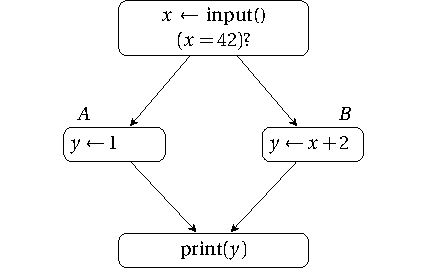
\includegraphics[scale=0.8]{ifthenelse-nonssa.pdf} \goto{CFG}{CFG}{0.8cm}

\end{minipage}
\begin{itemize}
\item multiple definitions of $y$ reach the print statement
\end{itemize}
~\vspace{3cm}
}%
\only<2>{\begin{minipage}{0.4\textwidth}
\begin{equation*}\small 
\begin{array}{l}
x = \texttt{input}();\\
\texttt{if } (x == 42)\\
\\
\texttt{then}\\
\quad    y_1 = 1;\\
\texttt{else}\\
\quad    y_2 = x + 2;\\
\texttt{end}\\
y_3 = \phi(y_1,y_2);\\
\texttt{print}(y_3);\\
\end{array}
\end{equation*}
\end{minipage}
\begin{minipage}{0.4\textwidth}
\strut
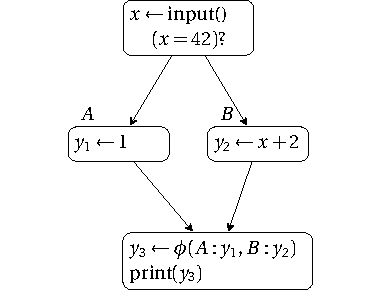
\includegraphics[scale=0.8]{ifthenelse-ssa.pdf}
\end{minipage}
\begin{itemize}
\item multiple definitions of $y$ are renamed as $y_1$ and $y_2$
\item $\phi$: merge values from different incoming paths\\ at control flow merge points
\end{itemize}
}
\end{frame}

\begin{frame}
\frametitle{Informal Semantics}
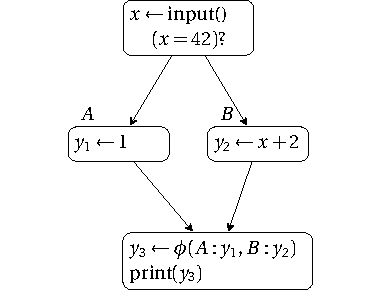
\includegraphics[scale=0.7]{ifthenelse-ssa.pdf}
\begin{minipage}[b]{0.5\textwidth}
\begin{itemize}
\item fixes the ambiguity; introduces $y_3$ which takes either $y_1$ or $y_2$
\item placed at control-flow merge points ie head of basic-blocks that have multiple predecessors
\end{itemize}
\end{minipage}
\begin{itemize}
\item $n$ parameters if it has $n$ incoming CFG path
\item optionaly can be represented as $a_0=\phi(B_1:a_1, \dots, B_n:a_n)$
\end{itemize}
\end{frame}

\begin{frame}
\frametitle{Informal Semantics}
\begin{itemize}
\item multiple $\phi$-functions executed simultaneously:\\ 
$
\begin{array}{l}
  a=\phi(a,b)\\
  b=\phi(b,a)
\end{array}
$
\item $\phi$-functions not directly executable (IR only: for static analysis)
\item removed before binary code generation (copy instructions)
\item exists extensions of $\phi$-functions (e.g. $\phi_{if}$, $\gamma$, etc.) that take an additional predicate parameter
\end{itemize}
\end{frame}

\begin{frame}
\frametitle{Informal Semantic}
\begin{minipage}[b]{\textwidth}
\begin{itemize}
\item SSA is not Dynamic Single Assignment (DSA or SA)
\item Construction: insert $\phi$-function where multiple reaching defs converged; version variables $x$ and $y$ (integer subscripts); 
\end{itemize}
\end{minipage}
\begin{minipage}[t]{0.5\textwidth}
\begin{equation*}\tiny
\begin{array}{l}
x = 0;\\
y = 0;\\
~\\\\\\\\
\texttt{while} (x < 10) \{\\
~\\\\\\
\quad  y = y + x;\\
\quad  x = x + 1;\\
\}\\
~\\\\
\texttt{print}(y)
\end{array} 
\end{equation*}
\end{minipage}
\begin{minipage}[t]{0.4\textwidth}
\strut
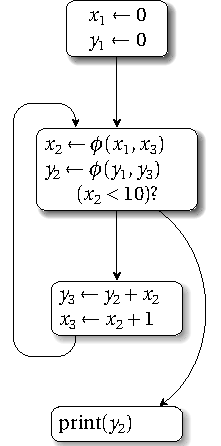
\includegraphics[valign=t,scale=0.65]{while}
\end{minipage}
\end{frame}

\begin{frame}
\frametitle{Comparison with Classical Data Flow Analysis}
\begin{itemize}
\item During actual program execution, information flows between variables
\item Static analysis captures this behavior by propagating abstract information along CFG
\item Can be propagated more efficiently using a functional or sparse representation such as SSA
\item constant propagation: definitions $\equiv$ set of points where information may change; associate information with variable names rather than variables $\times$ program points
%- other data flow problems can be accomodated by inserting additional pseudo-definition functions at appropriate points to induice renaming
\end{itemize}
\end{frame}

\begin{frame}
\frametitle{Comparison with Classical Data Flow Analysis}
\begin{block}{Null pointer analysis}
\only<1>{Determine statically if variable can contain null value at run-time\\~\vspace{3cm}}
\only<2->{\begin{tabular}[t]{cc}
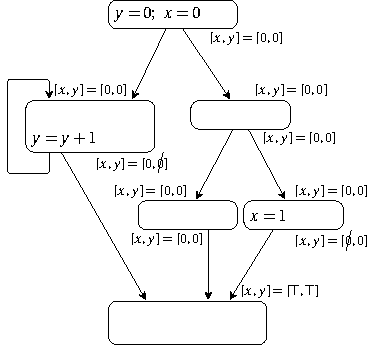
\includegraphics[valign=t,scale=0.6]{zero-1} &
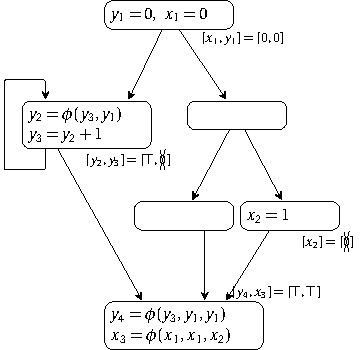
\includegraphics[valign=t,scale=0.6]{zero-2}\\
dense & SSA based
\end{tabular}}
\end{block}
\uncover<3>{
\begin{itemize}
\item Propagates from defs to uses (via def-use links); avoid program points where information does not change or not relevant
\item Results are more compact
\end{itemize}
}
\end{frame}

\begin{frame}
\frametitle{SSA in Context}
\begin{itemize} 
\item 1980s developments of IRs to encapsulate data dependences to expose direct link between definitions and uses (def-use chains). eg PDG, PD-web... SSA developed at IBM and published late 80s
\item GCC, Open64, HotSpot, Jikes, V8, Mono, LLVM... use SSA
\item more and more popular for JIT compilation on Java byte-code, CLI byte-code, LLVM bitcode...
\item because of favorable properties (simplification and reduced complexity) recently adopted back-end level even register allocation phase
\item also for high-level language impose referential transparency e.g. SISAL; on a per-variable basis final in Java, const or readonly in C\#. Immutability simplifies concurrent programming  
\end{itemize}
\end{frame}

\begin{frame}
\frametitle{Benefits of SSA}
\begin{itemize}
\item Compile time benefit (e.g. sparse data flow analysis)
\item Compiler development benefit (e.g. dead-code in GCC 4.x 40\% of GCC 3.x)
\item Program run-time benefit (simpler to develop more efficient analysis)
\end{itemize}
\begin{center}
\small
\begin{tabular}{p{0.45\textwidth}@{\kern.1\textwidth}p{0.43\textwidth}}
\hfil Myth\hfil & \hfil Reality \hfil \\ \hline
Greatly increases number of vars & $\approx$10\% expansion\\ [1ex]
Destruction generates many copy ops & not more than original prog. \\ [1ex]
SSA property difficult to maintain & $\equiv$ SSA construction restricted to some variables / code region 
\end{tabular}
\end{center}
\end{frame}


